\documentclass{article}

% content/resources/templates/preamble.tex
\usepackage[margin=0.6in]{geometry}
\author{Milav Dabgar}
\usepackage{amsmath,amssymb,amsthm}
\usepackage{booktabs}
\usepackage{multirow}
\usepackage{xcolor}
\usepackage{tcolorbox}
\tcbuselibrary{breakable,skins}
\usepackage[colorlinks=true,linkcolor=blue]{hyperref}
\usepackage{titlesec}
\usepackage{enumitem}
\usepackage{tikz}
\usepackage{pgfplots}
\usepackage{circuitikz}
\usepackage[version=4]{mhchem}
\usepackage{longtable}
\usepackage{array}
\usepackage{float}
\usepackage{caption}
\usepackage{listings}

\lstset{
  basicstyle=\small\ttfamily,
  breaklines=true,
  breakatwhitespace=false,
  postbreak=\mbox{\textcolor{red}{$\hookrightarrow$}\space},
  float=false,
  numbers=left,
  numberstyle=\tiny\color{gray},
  numbersep=10pt,
  xleftmargin=2em,
  keywordstyle=\color{blue},
  commentstyle=\color{green!60!black},
  stringstyle=\color{purple},
  backgroundcolor=\color{gray!5},
  showstringspaces=false,
  tabsize=2,
  captionpos=b,
  keepspaces=true,
  columns=flexible
}

\pgfplotsset{compat=1.18}
\usetikzlibrary{shapes,arrows,positioning,calc,patterns,decorations.pathmorphing,decorations.markings,arrows.meta}

% Color scheme
\definecolor{headcolor}{RGB}{0,102,204}
\definecolor{keycolor}{RGB}{220,20,60}
\definecolor{solutioncolor}{RGB}{34,139,34}
\definecolor{mnemoniccolor}{RGB}{148,0,211}
\definecolor{codecolor}{RGB}{0,0,100}

% Spacing
\setlength{\parskip}{3pt}
\setlist[itemize]{nosep}
\setlist[enumerate]{nosep}

% Title formatting
\titleformat{\section}{\Large\bfseries\color{headcolor}}{\thesection}{1em}{}
\titleformat{\subsection}{\large\bfseries\color{headcolor}}{\thesubsection}{1em}{}

% Pandoc tightlist compatibility
\providecommand{\tightlist}{%
  \setlength{\itemsep}{0pt}\setlength{\parskip}{0pt}}

% Pandoc longtable compatibility
\newcounter{none}
\def\thenone{}


% content/resources/templates/english-boxes.tex

% Custom environments
\newtcolorbox{solutionbox}{
 breakable,
 enhanced,
 colback=solutioncolor!5!white,
 colframe=solutioncolor!75!black,
 fonttitle=\bfseries,
 title=Solution
}

\newtcolorbox{solutionboxnobreak}{
 colback=solutioncolor!5!white,
 colframe=solutioncolor!75!black,
 fonttitle=\bfseries,
 title=Solution
}

\newtcolorbox{keyformula}{
 breakable,
 enhanced,
 colback=keycolor!5!white,
 colframe=keycolor!75!black,
 fonttitle=\bfseries,
 title=Key Formula
}

\newtcolorbox{mnemonicboxenv}{
 breakable,
 enhanced,
 colback=mnemoniccolor!5!white,
 colframe=mnemoniccolor!75!black,
 fonttitle=\bfseries,
 title=Mnemonic
}

\newcommand{\mnemonicbox}[1]{%
  \begin{mnemonicboxenv}
    #1
  \end{mnemonicboxenv}
}


% Custom commands for GTU solutions
% This file defines semantic commands for consistent formatting

% Question command with automatic formatting
\newcommand{\question}[2]{%
  \section*{Question #1}%
  \textbf{#2}%
}

% OR question variant
\newcommand{\questionor}[2]{%
  \section*{Question #1 OR}%
  \textbf{#2}%
}

% Proper table environment with caption
\newenvironment{answertable}[1]{%
  \begin{table}[htbp]
  \centering
  \caption{#1}
}{%
  \end{table}
}

% Proper figure environment for diagrams
\newenvironment{answerdiagram}[1]{%
  \begin{figure}[htbp]
  \centering
  \caption{#1}
}{%
  \end{figure}
}

% Semantic markup for key terms
\newcommand{\keyword}[1]{\textbf{#1}}
\newcommand{\code}[1]{\texttt{#1}}
\newcommand{\classname}[1]{\texttt{#1}}
\newcommand{\methodname}[1]{\texttt{#1}}

% Proper quotation marks
\newcommand{\mnemonic}[1]{``#1''}


\title{Electronic Measurements and Instruments (4331102) - Summer 2024 Solution}
\date{June 10, 2024}

\begin{document}
\maketitle

% Q1 Start
\questionmarks{1(a)}{3}{Define following term: (1) Accuracy (2) precision (3) Reproducibility}

\begin{solutionbox}
\begin{itemize}
    \item \keyword{Accuracy}: Closeness of measured value to the true value of measured quantity.
    \item \keyword{Precision}: Ability of an instrument to reproduce the same output for repeated applications of same input under identical conditions.
    \item \keyword{Reproducibility}: Degree of agreement between results of measurements of same quantity when measured under changed conditions (different method, observer, or time).
\end{itemize}
\end{solutionbox}

\begin{mnemonicbox}
\mnemonic{APR: Accurate-to-truth, Precise-repeats, Reproduce-under-change}
\end{mnemonicbox}

\questionmarks{1(b)}{4}{Explain construction of RTD Transducer with necessary diagram in detail. Also list application of it.}

\begin{solutionbox}
RTD (Resistance Temperature Detector) is a temperature sensor that operates on the principle that electrical resistance of metals changes with temperature.

\textbf{Diagram:}

\begin{center}
\begin{tikzpicture}[node distance=1.5cm, auto]
    \node [gtu block] (S) {Sensing Element};
    \node [gtu block, right=of S] (L) {Lead Wires};
    \node [gtu block, right=of L] (Sup) {Support};
    \node [gtu block, right=of Sup] (P) {Protective Sheath};
    
    \draw [gtu arrow] (S) -- (L);
    \draw [gtu arrow] (L) -- (Sup);
    \draw [gtu arrow] (Sup) -- (P);
\end{tikzpicture}
\captionof{figure}{RTD Construction Block Diagram}
\end{center}

\begin{itemize}
    \item \textbf{Sensing Element}: Pure platinum, nickel, or copper wire wound around ceramic core.
    \item \textbf{Lead Wires}: Connect RTD to measuring circuit.
    \item \textbf{Support}: Provides mechanical stability to sensing element.
    \item \textbf{Protective Sheath}: Protects sensing element from external environment.
\end{itemize}

\textbf{Applications of RTD:}
\begin{itemize}
    \item Temperature measurement in process industries.
    \item Food processing temperature monitoring.
    \item HVAC systems.
    \item Medical equipment.
\end{itemize}
\end{solutionbox}

\begin{mnemonicbox}
\mnemonic{RTD: Resistance Temperature Detector - Precise Temperature Measurement}
\end{mnemonicbox}

\questionmarks{1(c)}{7}{Explain working of Maxwell's Bridge with circuit diagram. List its advantages, disadvantages and applications.}

\begin{solutionbox}
Maxwell's Bridge is used to measure unknown inductance in terms of known capacitance and resistance.

\textbf{Circuit Diagram:}

\begin{center}
\begin{circuitikz}[american, scale=0.8, transform shape]
    \draw (0,4) coordinate(left) to[short, *-] (0,4);
    \draw (6,4) coordinate(right) to[short, *-] (6,4);
    \draw (3,7) coordinate(top) to[short, *-] (3,7);
    \draw (3,1) coordinate(bottom) to[short, *-] (3,1);

    % Arm 1 (Top-Left): Lx series Rx
    \draw (left) to[R, l=$R_1$] (0.5, 6) to[L, l=$L_1$] (top);

    % Arm 2 (Top-Right): R2
    \draw (top) to[R, l=$R_2$] (right);

    % Arm 3 (Bottom-Right): R3
    \draw (right) to[R, l=$R_3$] (bottom);

    % Arm 4 (Bottom-Left): R4 || C4
    \draw (bottom) -- (2.5, 2.5) to[R, l=$R_4$] (0.5, 4.5) -- (left);
    \draw (bottom) -- (1, 2) to[C, l=$C_4$] (-0.5, 3.5) -- (left);

    % Detector
    \draw (top) to[rmeter, t=D] (bottom);

    % Source
    \draw (left) to[short] (-2,4) to[short] (-2,0) to[battery1, l=$E$] (8,0) to[short] (8,4) to[short] (right);
\end{circuitikz}
\captionof{figure}{Maxwell's Inductance Capacitance Bridge}
\end{center}

\textbf{Working:}
At balance condition: $L_1 = C_4 \times R_2 \times R_3$

When the bridge is balanced, the detector shows zero current. The unknown inductance $L_1$ is calculated using above equation, where $C_4$ is known capacitance and $R_2, R_3$ are known resistances.

\begin{center}
\captionof{table}{Maxwell's Bridge Parameters}
\begin{tabulary}{\linewidth}{|L|L|}
\hline
\textbf{Parameter} & \textbf{Value} \\ \hline
Balance Equation & $L_1 = C_4 \times R_2 \times R_3$ \\ \hline
Quality Factor & $Q = \omega L_1/R_1 = \omega C_4 R_3$ \\ \hline
\end{tabulary}
\end{center}

\textbf{Advantages:}
\begin{itemize}
    \item High accuracy for medium Q inductors.
    \item Balance equations are independent of frequency.
    \item Simple calculation for inductance.
\end{itemize}

\textbf{Disadvantages:}
\begin{itemize}
    \item Not suitable for low Q inductor measurement.
    \item Requires variable standard capacitor.
    \item Affected by stray capacitance.
\end{itemize}

\textbf{Applications:}
\begin{itemize}
    \item Measuring inductance in laboratories.
    \item Calibration of inductance standards.
    \item Testing of inductive components.
\end{itemize}
\end{solutionbox}

\begin{mnemonicbox}
\mnemonic{Maxwell's Magic: Inductance equals Capacitance times Resistance squared}
\end{mnemonicbox}

\questionmarks{1(c) OR}{7}{Explain working of Wheatstone bridge with circuit diagram for balance condition. List its advantages, disadvantages, and applications.}

\begin{solutionbox}
Wheatstone bridge is used to measure unknown resistance by comparing it with known resistance values.

\textbf{Circuit Diagram:}

\begin{center}
\begin{circuitikz}[american, scale=0.8, transform shape]
    % Diamond structure
    \draw (0,3) coordinate(left) -- (3,6) coordinate(top) -- (6,3) coordinate(right) -- (3,0) coordinate(bottom) -- (0,3);
    
    % Resistors (clearing the path first)
    \draw (left) to[R, l=$P$, *-*] (top);
    \draw (top) to[R, l=$Q$, *-*] (right);
    \draw (right) to[R, l=$S$, *-*] (bottom);
    \draw (bottom) to[R, l=$R$, *-*] (left);
    
    % Galvanometer
    \draw (top) to[rmeter, t=G] (bottom);
    
    % Battery
    \draw (left) to[short] (-1,3) to[short] (-1,-1) to[battery1, l=$E$] (7,-1) to[short] (7,3) to[short] (right);
\end{circuitikz}
\captionof{figure}{Wheatstone Bridge Circuit}
\end{center}

\textbf{Working:}
At balance condition: $P/Q = R/S$ or $R = S \times (P/Q)$

When bridge is balanced, galvanometer shows zero deflection. Unknown resistance $R$ is calculated using the ratio of other resistances.

\begin{center}
\captionof{table}{Wheatstone Bridge Components}
\begin{tabulary}{\linewidth}{|L|L|}
\hline
\textbf{Component} & \textbf{Function} \\ \hline
$P, Q, S$ & Known resistances \\ \hline
$R$ & Unknown resistance \\ \hline
$G$ & Galvanometer (detector) \\ \hline
$E$ & DC voltage source \\ \hline
\end{tabulary}
\end{center}

\textbf{Advantages:}
\begin{itemize}
    \item High accuracy in resistance measurement.
    \item Simple construction and operation.
    \item Wide range of resistance measurement.
\end{itemize}

\textbf{Disadvantages:}
\begin{itemize}
    \item Cannot measure very low or very high resistances.
    \item Requires battery as power source.
    \item Temperature effects on resistors cause errors.
\end{itemize}

\textbf{Applications:}
\begin{itemize}
    \item Precise resistance measurement.
    \item Strain gauge measurements.
    \item Temperature sensing using RTDs.
    \item Transducer applications.
\end{itemize}
\end{solutionbox}

\begin{mnemonicbox}
\mnemonic{When WheatStone Balances: Product of opposites are equal ($P \times S = Q \times R$)}
\end{mnemonicbox}

% Q2 Start
\questionmarks{2(a)}{3}{Compare moving iron and moving coil type instruments.}

\begin{solutionbox}
\begin{center}
\captionof{table}{Moving Iron vs Moving Coil Instruments}
\begin{tabulary}{\linewidth}{|L|L|L|}
\hline
\textbf{Characteristic} & \textbf{Moving Iron Type} & \textbf{Moving Coil Type} \\ \hline
Principle & Magnetic attraction/repulsion & Electromagnetic force \\ \hline
Scale & Non-uniform (Cramped at beginning) & Uniform \\ \hline
Damping & Air friction damping (Poor) & Eddy current damping (Good) \\ \hline
Accuracy & Less accurate (2-5\%) & High accuracy (0.1-2\%) \\ \hline
Frequency range & DC and AC & DC only (without rectifier) \\ \hline
Power consumption & High & Low \\ \hline
Cost & Less expensive & More expensive \\ \hline
\end{tabulary}
\end{center}
\end{solutionbox}

\begin{mnemonicbox}
\mnemonic{IMAP-CAD: Iron-Magnetic-AC-Poor damping, Coil-Accurate-DC-Damped well}
\end{mnemonicbox}

\questionmarks{2(b)}{4}{Explain working and construction of successive approximation type DVM with necessary diagram.}

\begin{solutionbox}
Successive Approximation type Digital Voltmeter (DVM) converts analog voltage to digital value using binary search technique.

\textbf{Block Diagram:}
\begin{center}
\begin{tikzpicture}[node distance=1.5cm, auto]
    \node [gtu block] (SH) {Sample \& Hold};
    \node [gtu block, right=of SH] (Comp) {Comparator};
    \node [gtu block, right=of Comp, align=center] (SAR) {SAR Logic \&\\Register};
    \node [gtu block, below=of SAR] (DAC) {DAC};
    \node [gtu block, right=of SAR] (Disp) {Display};
    \node [coordinate, left=of SH] (In) {};
    
    \draw [gtu arrow] (In) -- node[above]{Input} (SH);
    \draw [gtu arrow] (SH) -- (Comp);
    \draw [gtu arrow] (Comp) -- (SAR);
    \draw [gtu arrow] (SAR) -- (DAC);
    \draw [gtu arrow] (DAC) -| (Comp);
    \draw [gtu arrow] (SAR) -- (Disp);
    
    \node [above=0.5cm of SAR] (Clk) {Clock};
    \draw [gtu arrow] (Clk) -- (SAR);
\end{tikzpicture}
\captionof{figure}{Successive Approximation DVM}
\end{center}

\textbf{Working:}
\begin{itemize}
    \item Sample \& Hold circuit captures input voltage.
    \item SAR sets MSB to 1, other bits to 0.
    \item DAC converts digital word to analog voltage.
    \item Comparator compares DAC output with input voltage.
    \item If DAC output $>$ Input, bit is reset to 0; otherwise kept 1.
    \item Process repeats for next bit until all bits are tested.
    \item Final digital word represents input voltage.
\end{itemize}

\textbf{Advantages:}
\begin{itemize}
    \item Medium conversion speed (10-100 $\mu$s).
    \item Good resolution and accuracy.
    \item Moderate cost.
\end{itemize}
\end{solutionbox}

\begin{mnemonicbox}
\mnemonic{SAR DVM: Sample-And-Register by Digital-Voltage-Matching}
\end{mnemonicbox}

\questionmarks{2(c)}{7}{1- A moving coil ammeter reading up to 10 amperes has a resistance of 0.02 ohm. How this instrument could be adopted to read current up to 1000 amperes? \\ 2- A moving coil voltmeter reading up to 200 mV has a resistance of 5 ohms. How this instrument can be adopted to read voltage up to 300 volts?}

\begin{solutionbox}
\textbf{Part 1: Ammeter Range Extension}

To extend ammeter range from 10A to 1000A, a shunt resistor is connected in parallel with the meter.

\textbf{Diagram:}
\begin{center}
\begin{circuitikz}[american, scale=0.8, transform shape]
    \draw (0,2) to[short, i=$I$] (1,2) coordinate(split);
    \draw (split) -- (1,3) to[R, l=$R_{sh}$, i=$I_{sh}$] (4,3) -- (4,2) coordinate(join);
    \draw (split) -- (1,1) to[rmeter, l=$R_m$, t=A, i=$I_m$] (4,1) -- (join);
    \draw (join) to[short] (5,2);
\end{circuitikz}
\captionof{figure}{Ammeter with Shunt}
\end{center}

\textbf{Calculation:}
\begin{itemize}
    \item Original meter resistance ($R_m$) = 0.02 $\Omega$
    \item Original full-scale current ($I_m$) = 10 A
    \item Desired full-scale current ($I$) = 1000 A
    \item Current through shunt ($I_{sh}$) = $I - I_m = 1000 - 10 = 990$ A
    \item Voltage across meter = Voltage across shunt
    \item $I_m \times R_m = I_{sh} \times R_{sh}$
    \item $R_{sh} = \frac{10 \times 0.02}{990} = \frac{0.2}{990} = 0.000202 \Omega$
\end{itemize}

\textbf{Part 2: Voltmeter Range Extension}

To extend voltmeter range from 200mV to 300V, a multiplier resistor is connected in series with the meter.

\textbf{Diagram:}
\begin{center}
\begin{circuitikz}[american, scale=0.8, transform shape]
    \draw (0,1) to[short, o-] (1,1) to[R, l=$R_s$] (3,1) to[rmeter, l=$R_m$, t=V] (5,1) to[short, -o] (6,1);
    \node at (0,1) [left] {+};
    \node at (6,1) [right] {-};
    \node at (3,0) {$V_{total}$};
\end{circuitikz}
\captionof{figure}{Voltmeter with Multiplier}
\end{center}

\textbf{Calculation:}
\begin{itemize}
    \item Original meter resistance ($R_m$) = 5 $\Omega$
    \item Original full-scale voltage ($V_m$) = 200 mV = 0.2 V
    \item Desired full-scale voltage ($V$) = 300 V
    \item Series resistance ($R_s$) = $R_m \times (\frac{V}{V_m} - 1)$
    \item $R_s = 5 \times (\frac{300}{0.2} - 1) = 5 \times (1500 - 1) = 5 \times 1499 = 7495 \Omega$
\end{itemize}
\end{solutionbox}

\begin{mnemonicbox}
\mnemonic{ShuntSeries: Shunt-for-Current, Series-for-Voltage}
\end{mnemonicbox}

\questionmarks{2(a) OR}{3}{Explain working and construction of Clamp on Meter with necessary diagram.}

\begin{solutionbox}
Clamp on Meter (Current Clamp) measures current without breaking the circuit by using electromagnetic induction.

\textbf{Diagram:}
\begin{center}
\begin{tikzpicture}[node distance=1.5cm, auto]
    \node [gtu block, align=center] (Clamp) {Clamp Jaw\\(Transformer Core)};
    \node [gtu block, below=of Clamp] (Rect) {Rectifier};
    \node [gtu block, below=of Rect] (ADC) {Measuring Ckt};
    \node [gtu block, below=of ADC] (Disp) {Display};
    \draw [thick] (Clamp.west) -- ++(-1,0) node[left] {Conductor};
    \draw [thick] (Clamp.east) -- ++(1,0) node[right] (current) {};
    
    \draw [gtu arrow] (Clamp) -- node[right]{Induced Current} (Rect);
    \draw [gtu arrow] (Rect) -- (ADC);
    \draw [gtu arrow] (ADC) -- (Disp);
\end{tikzpicture}
\captionof{figure}{Clamp Meter Block Diagram}
\end{center}

\textbf{Construction \& Working:}
\begin{itemize}
    \item \textbf{Clamp Jaw}: Split core transformer that can be opened to encircle conductor. Acts as secondary.
    \item \textbf{Current Transformer}: Converts primary current (in conductor) to proportional secondary current.
    \item \textbf{Rectifier}: Converts AC to DC for measurement circuit.
    \item \textbf{Measuring Circuit}: Processes signal and calculates current value.
    \item \textbf{Display}: Shows measured current value.
\end{itemize}
When a current-carrying conductor passes through the clamp jaw, it induces current in the secondary winding proportional to primary current, which is then measured.
\end{solutionbox}

\begin{mnemonicbox}
\mnemonic{CLAMP: Current-Loop Amplifies Magnetic Proportionally}
\end{mnemonicbox}

\questionmarks{2(b) OR}{4}{Explain working of PMMC instruments with necessary diagram.}

\begin{solutionbox}
PMMC (Permanent Magnet Moving Coil) instruments operate on the principle of electromagnetic force on current-carrying conductor in magnetic field.

\textbf{Diagram:}
\begin{center}
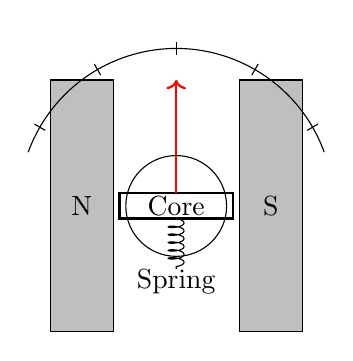
\begin{tikzpicture}[scale=0.8]
    % Magnets
    \draw[fill=lightgray] (-2,2) rectangle (-1,-2);
    \node at (-1.5,0) {N};
    \draw[fill=lightgray] (1,2) rectangle (2,-2);
    \node at (1.5,0) {S};
    
    % Core
    \draw (0,0) circle (0.8);
    \node at (0,0) {Core};
    
    % Coil (simplified)
    \draw[thick] (-0.9, -0.2) rectangle (0.9, 0.2);
    
    % Pointer
    \draw[->, thick, red] (0,0.2) -- (0,2);
    
    % Scale
    \draw (20:2.5) arc (20:160:2.5);
    \foreach \ang in {30,60,90,120,150}
        \draw (\ang:2.4) -- (\ang:2.6);
        
    % Springs (curly lines)
    \draw[decorate, decoration={coil, aspect=0.3, segment length=1mm, amplitude=1mm}] (0,-0.2) -- (0,-1);
    \node at (0,-1.2) {Spring};

\end{tikzpicture}
\captionof{figure}{PMMC Construction}
\end{center}

\textbf{Working:}
\begin{itemize}
    \item Current flows through rectangular coil placed in magnetic field.
    \item Electromagnetic force produces torque proportional to current ($T_d \propto I$).
    \item Spring provides controlling torque ($T_c \propto \theta$).
    \item Pointer deflects until $T_d = T_c$, so $\theta \propto I$.
    \item Damping system prevents oscillations.
\end{itemize}

\textbf{Components:}
\begin{itemize}
    \item Permanent magnet creates strong magnetic field.
    \item Soft iron core concentrates magnetic flux.
    \item Moving coil carries current to be measured.
    \item Control springs provide restoring force.
    \item Damping system (air or eddy current) reduces oscillations.
\end{itemize}
\end{solutionbox}

\begin{mnemonicbox}
\mnemonic{PMMC: Permanent Magnet Makes Current-proportional movement}
\end{mnemonicbox}

\questionmarks{2(c) OR}{7}{Draw the block diagram, working and construction of Integrating type DVM with necessary diagram and waveform.}

\begin{solutionbox}
Integrating type DVM (Digital Voltmeter) converts analog voltage to digital value by integrating the input over a fixed time.

\textbf{Block Diagram:}
\begin{center}
\begin{tikzpicture}[node distance=1.5cm, auto]
    \node [gtu block] (Int) {Integrator};
    \node [gtu block, right=of Int] (Comp) {Comparator};
    \node [gtu block, right=of Comp] (Logic) {Control Logic};
    \node [gtu block, below=of Logic] (Counter) {Counter};
    \node [gtu block, below=of Counter] (Disp) {Display};
    
    \node [coordinate, left=of Int] (In) {};
    \node [above=0.5cm of In] {Input $V_{in}$};
    \node [below=0.5cm of In] {Ref $V_{ref}$};
    
    % Switch logic simplified
    \draw [gtu arrow] (In) -- (Int); % Switch implied
    \draw [gtu arrow] (Int) -- (Comp);
    \draw [gtu arrow] (Comp) -- (Logic);
    \draw [gtu arrow] (Logic) -- (Counter);
    \draw [gtu arrow] (Counter) -- (Disp);
    \draw [gtu arrow] (Logic) -| (Int); % Control switch
    
    \node [above=0.5cm of Logic] (Osc) {Oscillator};
    \draw [gtu arrow] (Osc) -- (Logic);
\end{tikzpicture}
\captionof{figure}{Integrating DVM (Dual Slope)}
\end{center}

\textbf{Waveforms:}
\begin{center}
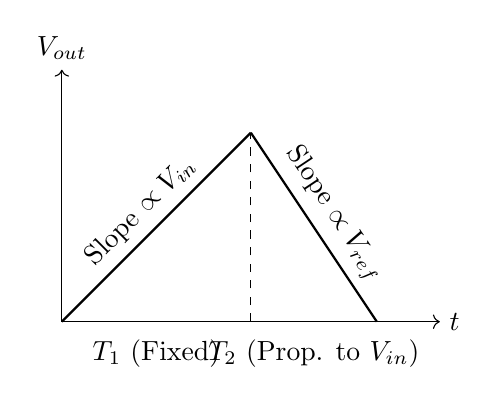
\begin{tikzpicture}[scale=0.8]
    \draw[->] (0,0) -- (6,0) node[right] {$t$};
    \draw[->] (0,0) -- (0,4) node[above] {$V_{out}$};
    
    % T1 Integration
    \draw[thick] (0,0) -- (3,3) node[midway, above, sloped] {Slope $\propto V_{in}$};
    \draw[dashed] (3,0) -- (3,3);
    \node at (1.5, -0.5) {$T_1$ (Fixed)};
    
    % T2 De-integration
    \draw[thick] (3,3) -- (5,0) node[midway, above, sloped] {Slope $\propto V_{ref}$};
    \draw[dashed] (5,0) -- (5,0); % Point
    \node at (4, -0.5) {$T_2$ (Prop. to $V_{in}$)};
    
\end{tikzpicture}
\captionof{figure}{Dual Slope Waveforms}
\end{center}

\textbf{Working:}
\begin{itemize}
    \item \textbf{Phase 1}: Integrate unknown voltage ($V_{in}$) for fixed time $T_1$. Capacitor charges.
    \item \textbf{Phase 2}: Integrate known reference voltage ($V_{ref}$) of opposite polarity until output reaches zero. Capacitor discharges.
    \item \textbf{Phase 3}: Counter counts clock pulses during phase 2 ($T_2$).
    \item $V_{in} = V_{ref} \times (T_2 / T_1)$.
\end{itemize}

\textbf{Advantages:}
\begin{itemize}
    \item High noise rejection.
    \item Good accuracy.
    \item Automatic zero adjustment.
\end{itemize}
\end{solutionbox}

\begin{mnemonicbox}
\mnemonic{Integrate-twice: Up with unknown, Down with reference}
\end{mnemonicbox}

% Q3 Start
\questionmarks{3(a)}{3}{In CRO What is the value of unknown DC voltage, if a straight line below x-axis is obtained with a displacement of 4cm and volt/div knob = 3V. calculate the unknown voltage Vdc.}

\begin{solutionbox}
\textbf{Calculation:}
\begin{itemize}
    \item Displacement = 4 cm (below x-axis)
    \item Volt/div setting = 3 V/div
    \item Direction = Below x-axis (negative voltage)
\end{itemize}

$$V_{dc} = -(\text{Displacement} \times \text{Volt/div})$$
$$V_{dc} = -(4 \text{ cm} \times 3 \text{ V/div})$$
$$V_{dc} = -12 \text{ V}$$

Therefore, the unknown DC voltage is \textbf{-12 V}.
\end{solutionbox}

\begin{mnemonicbox}
\mnemonic{voltage = Deflection \times Scale}
\end{mnemonicbox}

\questionmarks{3(b)}{4}{Draw internal structure of CRT. Explain in short.}

\begin{solutionbox}
CRT (Cathode Ray Tube) is the display device used in analog oscilloscopes.

\textbf{Diagram:}
\begin{center}
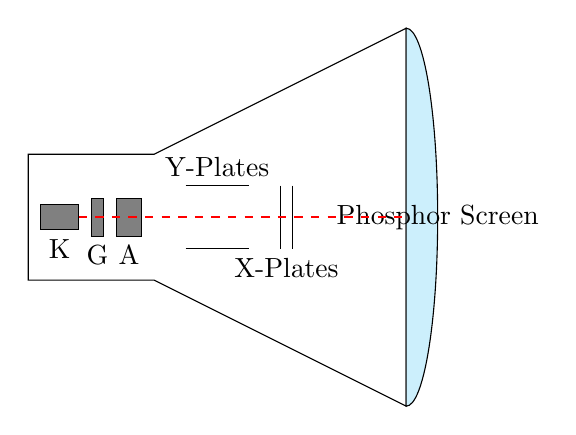
\begin{tikzpicture}[scale=0.8]
    % Glass envelope (funnel shape)
    \draw (0,1) -- (2,1) -- (6,3) -- (6,-3) -- (2,-1) -- (0,-1) -- cycle;
    
    % Screen
    \draw[fill=cyan!20] (6,3) arc (90:-90:0.5 and 3) -- cycle;
    \node at (6.5,0) {Phosphor Screen};
    
    % Electron Gun components
    \draw[fill=gray] (0.2,0.2) rectangle (0.8,-0.2); \node at (0.5,-0.5) {K}; % Cathode
    \draw[fill=gray] (1.0,0.3) rectangle (1.2,-0.3); \node at (1.1,-0.6) {G}; % Grid
    \draw[fill=gray] (1.4,0.3) rectangle (1.8,-0.3); \node at (1.6,-0.6) {A}; % Anodes
    
    % Deflection Plates
    \draw (2.5,0.5) -- (3.5,0.5); \draw (2.5,-0.5) -- (3.5,-0.5); \node at (3,0.8) {Y-Plates};
    \draw (4.0, 0.5) -- (4.0, -0.5); \draw (4.2, 0.5) -- (4.2, -0.5); \node at (4.1,-0.8) {X-Plates};
    
    % Electron Beam
    \draw[dashed, red, thick] (0.8,0) -- (6,0);
\end{tikzpicture}
\captionof{figure}{Internal Structure of CRT}
\end{center}

\textbf{Components:}
\begin{itemize}
    \item \textbf{Electron Gun}: Consists of heater, cathode, control grid, and anodes; produces electron beam.
    \item \textbf{Focusing System}: Focuses electron beam into sharp point using electrostatic lenses.
    \item \textbf{Deflection System}: Deflects electron beam horizontally and vertically using deflection plates.
    \item \textbf{Phosphor Screen}: Converts electron energy to visible light.
    \item \textbf{Glass Envelope}: Vacuum-sealed container housing all components.
\end{itemize}

\textbf{Working:}
\begin{itemize}
    \item Electron gun emits electrons.
    \item Focusing system narrows electron beam.
    \item Deflection plates move beam across screen.
    \item Beam strikes phosphor screen creating visible trace.
\end{itemize}
\end{solutionbox}

\begin{mnemonicbox}
\mnemonic{GFDS: Gun-Focus-Deflect-Screen}
\end{mnemonicbox}

\questionmarks{3(c)}{7}{Explain Construction, Block diagram, working and advantage of DSO with necessary diagram.}

\begin{solutionbox}
Digital Storage Oscilloscope (DSO) converts analog signals to digital form and stores them for display and analysis.

\textbf{Block Diagram:}
\begin{center}
\begin{tikzpicture}[node distance=1.5cm, auto]
    \node [gtu block] (Att) {Attenuator};
    \node [gtu block, right=of Att] (ADC) {ADC};
    \node [gtu block, right=of ADC] (Mem) {Memory};
    \node [gtu block, right=of Mem] (Micro) {Microprocessor};
    \node [gtu block, below=of Micro] (DAC) {DAC};
    \node [gtu block, left=of DAC] (Disp) {Display}; % Changed position for layout
    
    \node [coordinate, left=of Att] (In) {};
    \draw [gtu arrow] (In) -- node[above]{Input} (Att);
    
    \draw [gtu arrow] (Att) -- (ADC);
    \draw [gtu arrow] (ADC) -- (Mem);
    \draw [gtu arrow] (Mem) -- (Micro);
    \draw [gtu arrow] (Micro) -- (DAC);
    \draw [gtu arrow] (DAC) -- (Disp);
    
    \node [gtu block, above=of Micro] (CP) {Control Panel};
    \draw [gtu arrow] (CP) -- (Micro);
\end{tikzpicture}
\captionof{figure}{Digital Storage Oscilloscope Block Diagram}
\end{center}

\textbf{Construction and Working:}
\begin{itemize}
    \item \textbf{Input Stage}: Attenuator/amplifier conditions signal.
    \item \textbf{ADC}: Converts analog signal to digital at sampling rate.
    \item \textbf{Memory}: Stores digital samples.
    \item \textbf{Microprocessor}: Controls operation and processes data.
    \item \textbf{DAC}: Converts digital data back to analog for display.
    \item \textbf{Display}: Shows waveform.
\end{itemize}

\textbf{Advantages of DSO:}
\begin{itemize}
    \item Signal storage capability for later analysis.
    \item Pre-trigger viewing of signal.
    \item Single-shot signal capture.
    \item Automatic measurements and calculations.
    \item Waveform processing (FFT, averaging, etc.).
    \item Digital interfacing (USB, Ethernet).
\end{itemize}
\end{solutionbox}

\begin{mnemonicbox}
\mnemonic{SAMPLE: Store-Analyze-Measure-Process-Link-Examine}
\end{mnemonicbox}

\questionmarks{3(a) OR}{3}{In CRO vertical displacement for peak is = 1cm and volt/div knob = 10mV. Find peak value and RMS value of voltage.}

\begin{solutionbox}
\textbf{Calculation:}
\begin{itemize}
    \item Vertical displacement (peak) = 1 cm
    \item Volt/div setting = 10 mV/div
\end{itemize}

Peak value ($V_p$) = Displacement $\times$ Volt/div
$$V_p = 1 \text{ cm} \times 10 \text{ mV/div} = 10 \text{ mV}$$

For sinusoidal waveform:
RMS value ($V_{rms}$) = $V_p \div \sqrt{2}$
$$V_{rms} = 10 \text{ mV} \div 1.414 = 7.07 \text{ mV}$$

Therefore, \textbf{peak value = 10 mV} and \textbf{RMS value = 7.07 mV}.
\end{solutionbox}

\begin{mnemonicbox}
\mnemonic{Peak-to-RMS: Divide by root-2}
\end{mnemonicbox}

\questionmarks{3(b) OR}{4}{Explain CRO Screen in detail.}

\begin{solutionbox}
CRO (Cathode Ray Oscilloscope) screen displays waveforms and provides measurement references.

\textbf{Diagram:}
\begin{center}
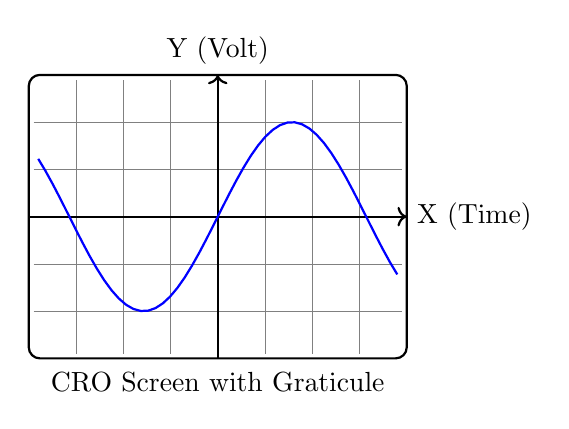
\begin{tikzpicture}[scale=0.6]
    % Screen bezel
    \draw[thick, rounded corners] (-4,-3) rectangle (4,3);
    
    % Graticule
    \draw[step=1cm, gray, very thin] (-3.9,-2.9) grid (3.9,2.9);
    
    % Axes
    \draw[thick, ->] (-4,0) -- (4,0) node[right] {X (Time)};
    \draw[thick, ->] (0,-3) -- (0,3) node[above] {Y (Volt)};
    
    % Trace
    \draw[blue, thick, domain=-3.8:3.8, samples=50] plot (\x, {2*sin(deg(\x))});
    
    \node at (0,-3.5) {CRO Screen with Graticule};
\end{tikzpicture}
\captionof{figure}{CRO Screen}
\end{center}

\textbf{Components:}
\begin{itemize}
    \item \textbf{Phosphor Coating}: Converts electron energy to visible light.
    \item \textbf{Graticule}: Grid pattern for measurements (typically $8 \times 10$ divisions).
    \item \textbf{X-Axis}: Represents time (horizontal).
    \item \textbf{Y-Axis}: Represents voltage (vertical).
    \item \textbf{Center Point}: Reference for measurements (0,0).
\end{itemize}

\textbf{Screen Features:}
\begin{itemize}
    \item \textbf{Divisions}: Subdivisions for precise reading.
    \item \textbf{Intensity Control}: Adjusts brightness of display.
    \item \textbf{Focus Control}: Sharpens displayed trace.
    \item \textbf{Scale Illumination}: Illuminates graticule.
\end{itemize}
\end{solutionbox}

\begin{mnemonicbox}
\mnemonic{PAXED: Phosphor-Axes-X-time-Y-amplitude-Equal-Divisions}
\end{mnemonicbox}

\questionmarks{3(c) OR}{7}{Explain Measurement of Voltage, Frequency, Time delay and Phase angle using CRO with necessary diagram.}

\begin{solutionbox}
CRO can measure various electrical parameters accurately.

\textbf{1. Voltage Measurement:}
\begin{center}
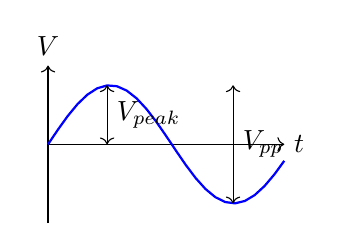
\begin{tikzpicture}[scale=0.5]
    \draw[->] (0,0) -- (6,0) node[right] {$t$};
    \draw[->] (0,-2) -- (0,2) node[above] {$V$};
    \draw[thick, blue] plot[domain=0:6] (\x, {1.5*sin(deg(\x))});
    \draw[<->] (1.5,0) -- (1.5,1.5) node[midway, right] {$V_{peak}$};
    \draw[<->] (4.7,-1.5) -- (4.7,1.5) node[midway, right] {$V_{pp}$};
\end{tikzpicture}
\end{center}
\begin{itemize}
    \item Count vertical divisions of waveform.
    \item Multiply by V/div setting.
    \item Amplitude = Vertical divisions $\times$ V/div.
\end{itemize}

\textbf{2. Frequency Measurement:}
\begin{center}
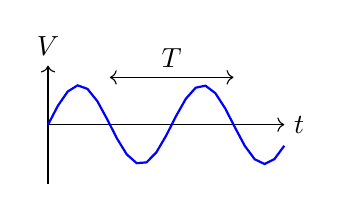
\begin{tikzpicture}[scale=0.5]
    \draw[->] (0,0) -- (6,0) node[right] {$t$};
    \draw[->] (0,-1.5) -- (0,1.5) node[above] {$V$};
    \draw[thick, blue] plot[domain=0:6] (\x, {sin(deg(2*\x))});
    \draw[<->] (1.57, 1.2) -- (4.71, 1.2) node[midway, above] {$T$};
\end{tikzpicture}
\end{center}
\begin{itemize}
    \item Measure time period ($T$) between similar points.
    \item Frequency $f = 1/T$.
    \item $T = \text{Horizontal divisions} \times \text{Time/div}$.
\end{itemize}

\textbf{3. Time Delay \& 4. Phase Angle Measurement:}
\begin{center}
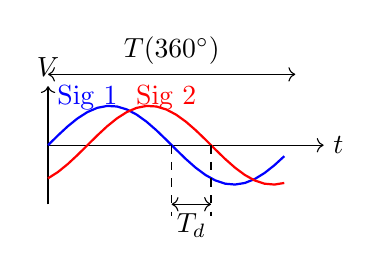
\begin{tikzpicture}[scale=0.5]
    \draw[->] (0,0) -- (7,0) node[right] {$t$};
    \draw[->] (0,-1.5) -- (0,1.5) node[above] {$V$};
    
    % Signal 1
    \draw[thick, blue] plot[domain=0:6] (\x, {sin(deg(\x))});
    \node[blue] at (1, 1.2) {Sig 1};
    
    % Signal 2 (Shifted)
    \draw[thick, red] plot[domain=0:6] (\x, {sin(deg(\x - 1))});
    \node[red] at (3, 1.2) {Sig 2};
    
    % Drawing delay
    \draw[dashed] (3.14, 0) -- (3.14, -1.8);
    \draw[dashed] (4.14, 0) -- (4.14, -1.8);
    \draw[<->] (3.14, -1.5) -- (4.14, -1.5) node[midway, below] {$T_d$};
    
    % Period T
    \draw[<->] (0, 1.8) -- (6.28, 1.8) node[midway, above] {$T (360^\circ)$};
\end{tikzpicture}
\end{center}
\begin{itemize}
    \item \textbf{Time Delay}: Measure horizontal distance ($T_d$) between corresponding points of two signals.
    \item \textbf{Phase Angle}:
    \begin{itemize}
        \item Measure time period ($T$) of one complete cycle.
        \item Measure time delay ($T_d$).
        \item Phase angle $\phi = (T_d/T) \times 360^\circ$.
    \end{itemize}
\end{itemize}
\end{solutionbox}

\begin{mnemonicbox}
\mnemonic{VFTP: Vertical-Frequency-Time-Phase}
\end{mnemonicbox}


% Q4 Start
\questionmarks{4(a)}{3}{Compare active and passive transducers.}

\begin{solutionbox}
\begin{center}
\captionof{table}{Active vs Passive Transducers}
\begin{tabulary}{\linewidth}{|L|L|L|}
\hline
\textbf{Characteristic} & \textbf{Active Transducers} & \textbf{Passive Transducers} \\ \hline
Power source & Self-generating (no external power) & Requires external power \\ \hline
Output & Generates energy from input & Modifies external energy \\ \hline
Examples & Thermocouple, Photovoltaic cell & Strain gauge, RTD, LVDT \\ \hline
Sensitivity & Generally lower & Generally higher \\ \hline
Response time & Faster & Slower \\ \hline
Cost & Usually less expensive & Usually more expensive \\ \hline
Complexity & Simpler & More complex \\ \hline
\end{tabulary}
\end{center}
\end{solutionbox}

\begin{mnemonicbox}
\mnemonic{APE-GSR: Active-Produces-Energy, Gets-Signal-Requiring-power}
\end{mnemonicbox}

\questionmarks{4(b)}{4}{Explain Working of strain Gauge with necessary diagram in detail. Also list application of it.}

\begin{solutionbox}
Strain gauge converts mechanical deformation to electrical resistance change.

\textbf{Diagram:}
\begin{center}
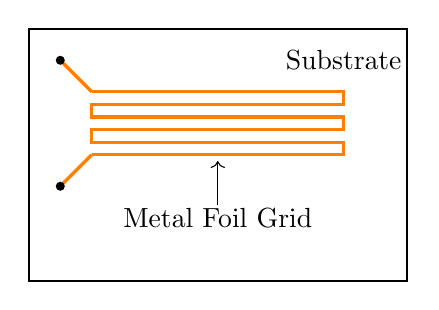
\begin{tikzpicture}[scale=0.8]
    \draw[thick] (0,0) -- (6,0) -- (6,4) -- (0,4) -- cycle; % Substrate
    \node at (5,3.5) {Substrate};
    
    % Wire grid
    \draw[very thick, orange] (1,3) -- (5,3) -- (5,2.8) -- (1,2.8) -- (1,2.6) -- (5,2.6) -- (5,2.4) -- (1,2.4) -- (1,2.2) -- (5,2.2) -- (5,2) -- (1,2);
    
    % Terminals
    \draw[very thick, orange] (1,3) -- (0.5,3.5); \node[draw, circle, inner sep=1pt, fill=black] at (0.5,3.5) {};
    \draw[very thick, orange] (1,2) -- (0.5,1.5); \node[draw, circle, inner sep=1pt, fill=black] at (0.5,1.5) {};
    
    \node at (3,1) {Metal Foil Grid};
    \draw[->] (3,1.2) -- (3,1.9);
\end{tikzpicture}
\captionof{figure}{Strain Gauge Construction}
\end{center}

\textbf{Working:}
\begin{itemize}
    \item When a conductor is stretched, its length increases and cross-sectional area decreases.
    \item This causes an increase in electrical resistance: $\Delta R/R = GF \times \epsilon$.
    \item Where $\Delta R/R$ is fractional change in resistance, $GF$ is gauge factor, $\epsilon$ is strain.
\end{itemize}

\textbf{Applications:}
\begin{itemize}
    \item Load cells for weighing systems.
    \item Structural health monitoring.
    \item Pressure sensors.
    \item Torque measurement.
    \item Mechanical stress analysis.
\end{itemize}
\end{solutionbox}

\begin{mnemonicbox}
\mnemonic{STRAIN: Stretch-To-Resistance-Alteration-In-Narrow-conductor}
\end{mnemonicbox}

\questionmarks{4(c)}{7}{Explain Gas Sensor MQ2 with necessary diagram in detail.}

\begin{solutionbox}
MQ2 is a semiconductor gas sensor that detects combustible gases, smoke, and LPG.

\textbf{Diagram:}
\begin{center}
\begin{tikzpicture}[node distance=1.5cm, auto]
    \node [gtu block] (SnO2) {SnO$_2$ Sensing Element};
    \node [gtu block, below=of SnO2] (Heater) {Heater Coil};
    \node [gtu block, left=of SnO2] (Anti) {Anti-explosion Net};
    \node [gtu block, right=of SnO2] (Elec) {Electrodes};
    
    \node [draw, dashed, fit=(SnO2) (Heater) (Anti) (Elec), label=above:Housing] (Housing) {};
\end{tikzpicture}
\captionof{figure}{MQ2 Sensor Structure}
\end{center}

\textbf{Construction:}
\begin{itemize}
    \item \textbf{Sensing Element}: Tin dioxide (SnO$_2$) semiconductor.
    \item \textbf{Heater}: Maintains operating temperature (around 200-400$^\circ$C).
    \item \textbf{Electrodes}: Measure resistance changes.
    \item \textbf{Housing}: Protects components and allows gas flow.
\end{itemize}

\textbf{Working Principle:}
\begin{itemize}
    \item In clean air, sensor has high resistance.
    \item When combustible gases present, surface reactions occur.
    \item Electrons are released, decreasing resistance.
    \item Resistance decreases proportionally to gas concentration.
\end{itemize}

\textbf{Circuit Connection:}
\begin{center}
\begin{circuitikz}[american, scale=0.8, transform shape]
    \draw (0,4) node[above] {$V_{cc} (+5V)$} to[short, o-] (0,3) to[R, l=$R_{load}$] (0,1) to[short] (2,1) to[short] (2,3) to[short] (0,3);
    \draw (2,3) -- (4,3) to[vR, l=MQ2] (4,1) -- (2,1); % Conceptual representation
    \draw (0,1) to[short, -o] (0,0) node[below] {$V_{out}$};
    \draw (4,1) node[ground]{};
    \node at (3,2) {Sensor};
\end{circuitikz}
\captionof{figure}{Basic MQ2 Circuit}
\end{center}
\end{solutionbox}

\begin{mnemonicbox}
\mnemonic{MQ2: Measures Quick-leaks of 2+ gases (LPG, Propane)}
\end{mnemonicbox}

\questionmarks{4(a) OR}{3}{Compare primary and secondary transducers}

\begin{solutionbox}
\begin{center}
\captionof{table}{Primary vs Secondary Transducers}
\begin{tabulary}{\linewidth}{|L|L|L|}
\hline
\textbf{Characteristic} & \textbf{Primary Transducers} & \textbf{Secondary Transducers} \\ \hline
Definition & Directly convert physical quantity to electrical signal & Convert output of primary transducer to usable form \\ \hline
Function & First stage of conversion & Second stage of conversion \\ \hline
Examples & Thermocouple, Photocell, Piezoelectric & Amplifiers, ADCs, Signal conditioners \\ \hline
Input & Physical parameter & Output from primary transducer \\ \hline
Output & Electrical signal & Modified electrical signal \\ \hline
Location & At sensing point & May be remote from primary transducer \\ \hline
Accuracy & Affects overall system accuracy & Further processes already converted signal \\ \hline
\end{tabulary}
\end{center}
\end{solutionbox}

\begin{mnemonicbox}
\mnemonic{PS-FLIP: Primary-Senses, Secondary-Further-Level-Improves-Processing}
\end{mnemonicbox}

\questionmarks{4(b) OR}{4}{Explain Capacitive Transducer with necessary diagram in detail. Also list application of it.}

\begin{solutionbox}
Capacitive transducer converts physical displacement into capacitance change which is then converted to electrical signal.

\textbf{Diagram:}
\begin{center}
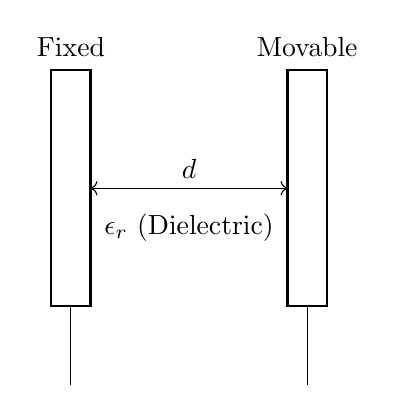
\begin{tikzpicture}
    % Plate 1
    \draw[thick] (0,0) rectangle (0.5, 3); \node at (0.25, 3.3) {Fixed};
    % Plate 2
    \draw[thick] (3,0) rectangle (3.5, 3); \node at (3.25, 3.3) {Movable};
    % Distance d
    \draw[<->] (0.5, 1.5) -- (3, 1.5) node[midway, above] {$d$};
    % Area A implied
    % Leads
    \draw (0.25, 0) -- (0.25, -1);
    \draw (3.25, 0) -- (3.25, -1);
    
    \node at (1.75, 1) {$\epsilon_r$ (Dielectric)};
\end{tikzpicture}
\captionof{figure}{Capacitive Transducer Principle}
\end{center}

\textbf{Working:}
$$C = \frac{\epsilon_0 \epsilon_r A}{d}$$
Where $\epsilon_0$ is permittivity of free space, $\epsilon_r$ is relative permittivity, $A$ is area, $d$ is distance.

Capacitance changes by:
\begin{itemize}
    \item Varying distance between plates ($d$).
    \item Varying overlap area of plates ($A$).
    \item Varying dielectric constant ($\epsilon_r$).
\end{itemize}

\textbf{Applications:}
\begin{itemize}
    \item Pressure sensors.
    \item Displacement measurements.
    \item Level indicators.
    \item Humidity sensors.
    \item Touch screens.
\end{itemize}
\end{solutionbox}

\begin{mnemonicbox}
\mnemonic{CAPACITIVE: Change-Area-Plates-And-Change-In-Thickness-Impacts-Value-Electrically}
\end{mnemonicbox}

\questionmarks{4(c) OR}{7}{Explain LVDT Transducer operation, construction with necessary diagram in detail. Also list advantage, disadvantage and application of LVDT.}

\begin{solutionbox}
LVDT (Linear Variable Differential Transformer) is an electromagnetic transducer that converts linear displacement to electrical signal.

\textbf{Diagram:}
\begin{center}
\begin{circuitikz}[american, scale=0.8, transform shape]
    % Core
    \draw[fill=gray!30] (2,1.5) rectangle (4,2.5);
    \node at (3,2) {Core};
    \draw[<->] (2.5, 2.7) -- (3.5, 2.7) node[midway, above] {Motion};
    
    % Primary
    \draw[decorate, decoration={coil, segment length=5pt, amplitude=5pt}] (2,0) -- (4,0);
    \node at (3,-0.5) {Primary (P)};
    \draw (2,0) to[short, -o] (2,-1); \draw (4,0) to[short, -o] (4,-1);
    \node at (3,-1) {$V_{in}$ (AC)};
    
    % Secondaries
    \draw[decorate, decoration={coil, segment length=5pt, amplitude=5pt}] (0,1.5) -- (0,3.5);
    \node at (-0.5, 2.5) {S1};
    \draw[decorate, decoration={coil, segment length=5pt, amplitude=5pt}] (6,1.5) -- (6,3.5);
    \node at (6.5, 2.5) {S2};
    
    % Connections
    \draw (0,1.5) to[short] (2, 1.5); % Just illustrative
    % Let's draw schematic standard
\end{circuitikz}
\begin{circuitikz}[american, scale=0.8, transform shape]
    \node [transformer core] (T) {};
    % This is too simple. Manual draw.
    
    % Primary
    \draw (0,0) to[L, l=P] (0,2);
    % Secondaries S1, S2
    \draw (2,2) to[L, l=S1] (2,1) -- (2,1) to[L, l=S2] (2,0);
    
    % Core
    \draw[thick] (0.8,-0.2) -- (0.8,2.2);
    \draw[thick] (1.2,-0.2) -- (1.2,2.2);
    \node at (1, 2.5) {Core};
    \draw[<->] (1, -0.5) -- (1, -1) node[right] {Disp};
    
    % Series Opposition
    \draw (2,2) -- (3,2) to[short, -o] (4,2);
    \draw (2,0) -- (3,0) to[short, -o] (4,0);
    \node at (4.5,1) {$V_{out} = V_{s1} - V_{s2}$};
\end{circuitikz}
\captionof{figure}{LVDT Schematic}
\end{center}

\textbf{Construction:}
\begin{itemize}
    \item \textbf{Primary Coil}: Center coil excited by AC source.
    \item \textbf{Secondary Coils}: Two coils connected in series opposition.
    \item \textbf{Core}: Ferromagnetic material that moves with measured displacement.
    \item \textbf{Housing}: Protects the coil assembly.
\end{itemize}

\textbf{Working:}
\begin{itemize}
    \item AC excitation applied to primary coil.
    \item At null position (center), equal voltages induced in S1, S2 ($V_{out} = 0$).
    \item Moving core towards S1 increases $V_{s1}$, decreasing $V_{s2}$ ($V_{out} = V_{s1} - V_{s2}$).
    \item Phase indicates direction.
\end{itemize}

\textbf{Advantages:} Non-contact, High resolution, Robust.
\textbf{Disadvantages:} AC source needed, Costly.
\textbf{Applications:} Position feedback, Robotics, Aircraft control.
\end{solutionbox}

\begin{mnemonicbox}
\mnemonic{LVDT: Linear-Variation-Detected-Through electromagnetic induction}
\end{mnemonicbox}

% Q5 Start
\questionmarks{5(a)}{3}{Explain working of Thermocouple sensor with necessary diagram in detail.}

\begin{solutionbox}
Thermocouple is a temperature sensor based on the Seebeck effect.

\textbf{Diagram:}
\begin{center}
\begin{circuitikz}[american, scale=0.8, transform shape]
    \draw (0,0) coordinate(Cold) to[short] (0, 0.5) to[R, l=Metal A] (4, 0.5) to[short] (4,0) coordinate(Hot);
    \draw (Hot) to[short] (4, -0.5) to[R, l=Metal B] (0, -0.5) to[short] (Cold);
    
    \node [left] at (Cold) {Cold Junction ($T_1$)};
    \node [right] at (Hot) {Hot Junction ($T_2$)};
    
    % Voltmeter at cold junction usually open
    % Let's redraw
    \draw (-2, 1) coordinate(Vpos) to[R, l=Metal A] (2,1) coordinate(J1);
    \draw (-2, -1) coordinate(Vneg) to[R, l=Metal B] (2,-1) coordinate(J1_end); % Wait
    % Standard diagram:
    % Junction 1 (Hot)
    \draw (4,0) circle (0.1) node[right]{Hot};
    \draw (4,0) -- (0,1) node[left]{Metal A};
    \draw (4,0) -- (0,-1) node[left]{Metal B};
    \draw (0,1) to[rmeter, t=V] (0,-1);
    \node at (0,0.5) {Cold Junction}; % This is actually Reference
\end{circuitikz}
\captionof{figure}{Thermocouple Circuit}
\end{center}
\textbf{Working:}
\begin{itemize}
    \item Two dissimilar metals joined at two points.
    \item Temperature difference ($T_2 - T_1$) creates Seebeck voltage (EMF).
    \item $E \propto (T_2 - T_1)$.
\end{itemize}
\end{solutionbox}

\begin{mnemonicbox}
\mnemonic{THC: Temperature-produces Hot-junction Current}
\end{mnemonicbox}

\questionmarks{5(b)}{4}{Explain working of Digital IC tester with necessary diagram in detail.}

\begin{solutionbox}
Digital IC Tester tests functionality of digital ICs by applying test vectors.

\textbf{Block Diagram:}
\begin{center}
\begin{tikzpicture}[node distance=1.5cm, auto]
    \node [gtu block] (Ctrl) {Control Unit};
    \node [gtu block, right=of Ctrl] (Gen) {Vector Gen};
    \node [gtu block, right=of Gen] (CUT) {IC Under Test};
    \node [gtu block, right=of CUT] (Resp) {Response Analyzer};
    \node [gtu block, below=of Resp] (Disp) {Display};
    \node [gtu block, below=of Ctrl] (UI) {User Interface};
    
    \draw [gtu arrow] (UI) -- (Ctrl);
    \draw [gtu arrow] (Ctrl) -- (Gen);
    \draw [gtu arrow] (Gen) -- (CUT);
    \draw [gtu arrow] (CUT) -- (Resp);
    \draw [gtu arrow] (Resp) -- (Disp);
    \draw [gtu arrow] (Ctrl) -| (Disp);
\end{tikzpicture}
\captionof{figure}{IC Tester Block Diagram}
\end{center}

\textbf{Working:}
\begin{itemize}
    \item \textbf{Control Unit}: Manages testing process.
    \item \textbf{Vector Generator}: Applies input patterns to IC pins.
    \item \textbf{IC Under Test}: The component being verified.
    \item \textbf{Response Analyzer}: Compares output with expected truth table.
    \item \textbf{Display}: Shows PASS/FAIL.
\end{itemize}
\end{solutionbox}

\begin{mnemonicbox}
\mnemonic{VECTOR: Verify-Each-Circuit-Through-Output-Response}
\end{mnemonicbox}

\questionmarks{5(c)}{7}{Explain working of function generator with necessary diagram in detail.}

\begin{solutionbox}
Function generator produces different waveforms (sine, square, triangle).

\textbf{Block Diagram:}
\begin{center}
\begin{tikzpicture}[node distance=1.3cm, auto]
    \node [gtu block] (Freq) {Freq Control};
    \node [gtu block, right=of Freq] (Osc) {Oscillator (Triangle/Square)};
    \node [gtu block, right=of Osc] (Shape) {Wave Shaper (Sine)};
    \node [gtu block, below=of Shape] (Sel) {Selector Switch};
    \node [gtu block, left=of Sel] (Att) {Attenuator};
    \node [gtu block, left=of Att] (Amp) {Output Amp};
    
    \draw [gtu arrow] (Freq) -- (Osc);
    \draw [gtu arrow] (Osc) -- (Shape);
    \draw [gtu arrow] (Osc) -- (Sel); % Square/Triangle direct
    \draw [gtu arrow] (Shape) -- (Sel); % Sine
    \draw [gtu arrow] (Sel) -- (Att);
    \draw [gtu arrow] (Att) -- (Amp);
    \draw [gtu arrow] (Amp) -- ++(-1.5,0) node[left]{Output};
\end{tikzpicture}
\captionof{figure}{Function Generator Block Diagram}
\end{center}

\textbf{Working:}
\begin{itemize}
    \item \textbf{Oscillator}: Generates basic Triangle and Square waves.
    \item \textbf{Wave Shaper}: Converts Triangle to Sine wave using diode shaping.
    \item \textbf{Selector}: Selects desired waveform.
    \item \textbf{Attenuator/Amp}: Controls amplitude and output impedance.
\end{itemize}
\end{solutionbox}

\begin{mnemonicbox}
\mnemonic{FAST: Frequency-Amplitude-Signal-Type control}
\end{mnemonicbox}

\questionmarks{5(a) OR}{3}{Explain working of PH sensor with necessary diagram in detail.}

\begin{solutionbox}
PH sensor measures hydrogen ion concentration.

\textbf{Diagram:}
\begin{center}
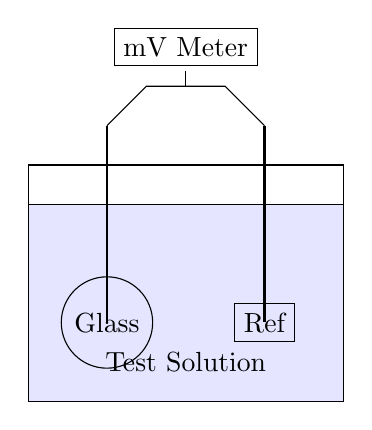
\begin{tikzpicture}
    % Beaker
    \draw (0,0) -- (0,3) -- (4,3) -- (4,0) -- cycle;
    \draw[fill=blue!10] (0,0) rectangle (4,2.5);
    \node at (2,0.5) {Test Solution};
    
    % Electrodes
    \draw[thick] (1, 3.5) -- (1, 1); \node[draw, circle] at (1,1) {Glass};
    \draw[thick] (3, 3.5) -- (3, 1); \node[draw, rectangle] at (3,1) {Ref};
    
    % Meter
    \draw (1, 3.5) -- (1.5, 4) -- (2.5, 4) -- (3, 3.5);
    \node[draw, rectangle] at (2, 4.5) {mV Meter};
    \draw (2, 4) -- (2, 4.2);
\end{tikzpicture}
\captionof{figure}{pH Measurement System}
\end{center}

\textbf{Working:}
\begin{itemize}
    \item Glass electrode contains buffer solution.
    \item Potential difference develops across glass membrane due to H$^+$ ion difference.
    \item Voltage is proportional to pH (59.16 mV/pH).
\end{itemize}
\end{solutionbox}

\begin{mnemonicbox}
\mnemonic{pH-MVH: Potential-of-Hydrogen Measured by Voltage per Hydrogen-ion concentration}
\end{mnemonicbox}

\questionmarks{5(b) OR}{4}{Describe working of Spectrum Analyzer with necessary diagram in detail}

\begin{solutionbox}
Spectrum Analyzer displays signal amplitude vs. frequency.

\textbf{Block Diagram:}
\begin{center}
\begin{tikzpicture}[node distance=1.5cm, auto]
    \node [gtu block] (Mix) {Mixer};
    \node [gtu block, right=of Mix] (IF) {IF Filter};
    \node [gtu block, right=of IF] (Det) {Detector};
    \node [gtu block, right=of Det] (Disp) {Display};
    
    \node [gtu block, below=of Mix] (LO) {Local Osc};
    \node [gtu block, right=of LO] (Sweep) {Sweep Gen};
    
    \node [coordinate, left=of Mix] (In) {};
    \draw [gtu arrow] (In) -- node[above]{Input} (Mix);
    \draw [gtu arrow] (Mix) -- (IF);
    \draw [gtu arrow] (IF) -- (Det);
    \draw [gtu arrow] (Det) -- (Disp);
    
    \draw [gtu arrow] (LO) -- (Mix);
    \draw [gtu arrow] (Sweep) -- (LO);
    \draw [gtu arrow] (Sweep) -| (Disp); % X-deflection
\end{tikzpicture}
\captionof{figure}{Spectrum Analyzer Block Diagram}
\end{center}

\textbf{Working:}
\begin{itemize}
    \item \textbf{Mixer}: Mixes input with swept Local Oscillator (LO).
    \item \textbf{IF Filter}: Selects specific frequency component.
    \item \textbf{Detector}: Converts IF magnitude to DC (Y-axis).
    \item \textbf{Sweep Gen}: Sweeps LO frequency and drives X-axis.
\end{itemize}
\end{solutionbox}

\begin{mnemonicbox}
\mnemonic{SAFE-D: Signal-Amplitude-Frequency-Evaluation-Display}
\end{mnemonicbox}

\questionmarks{5(c) OR}{7}{Explain working of basic frequency counter with necessary diagram in detail}

\begin{solutionbox}
Frequency counter measures frequency by counting cycles in a fixed time.

\textbf{Block Diagram:}
\begin{center}
\begin{tikzpicture}[node distance=1.5cm, auto]
    \node [gtu block] (Cond) {Input Cond};
    \node [gtu block, right=of Cond] (Trig) {Schmitt Trig};
    \node [gtu block, right=of Trig] (Gate) {AND Gate};
    \node [gtu block, right=of Gate] (Counter) {Counter};
    \node [gtu block, right=of Counter] (Disp) {Display};
    
    \node [gtu block, below=of Gate] (TB) {Time Base};
    \node [coordinate, left=of Cond] (In) {};
    
    \draw [gtu arrow] (In) -- (Cond);
    \draw [gtu arrow] (Cond) -- (Trig);
    \draw [gtu arrow] (Trig) -- (Gate);
    \draw [gtu arrow] (Gate) -- (Counter);
    \draw [gtu arrow] (Counter) -- (Disp);
    \draw [gtu arrow] (TB) -- (Gate);
\end{tikzpicture}
\captionof{figure}{Frequency Counter Block Diagram}
\end{center}

\textbf{Working:}
\begin{itemize}
    \item \textbf{Input Conditioning}: Shapes signal.
    \item \textbf{Schmitt Trigger}: Converts to square pulses.
    \item \textbf{Time Base}: Opens Main Gate for precise time (T).
    \item \textbf{Counter}: Counts pulses ($N$) when gate is open.
    \item Frequency $f = N/T$.
\end{itemize}
\end{solutionbox}

\begin{mnemonicbox}
\mnemonic{COUNT: Cycles-Over-Unit-time-Numerically-Tallied}
\end{mnemonicbox}

\end{document}

